\section{Memory-Related Performance Problems}\label{sec:background}
As modern computing systems evolve, the demand for increased computational power and memory resources has become more prevalent. This demand is driven by the increasing complexity of applications and the need to process larger amounts of data. In this section, we will explore the challenges and performance problems that result from the ever-growing requirements for memory and computational resources. We begin by discussing the processor-memory performance gap and its implications in Section \ref{sec:pmgap}, followed by a brief examination of the increasing computational and memory requirements of modern applications (Section \ref{sec:comp_mem_req}). The processor-memory performance gap and the increasing computational and memory requirements combined result in a need to tackle high data transfer costs and bottlenecks (Section \ref{sec:data_transfer}). Finally, we will define the concept of data locality in Section \ref{sec:data_locality}, which solutions consider to the aforementioned problems.

\subsection{Processor-Memory Performance Gap}\label{sec:pmgap}
It is well known, that the performance of CPUs doubles roughly every two years, a phenomenon resulting from Moore's law. Similarly, memory technology has also been progressing exponentially, however, at a slower pace \cite{efnusheva2017survey, machanick2002approaches, mckee2004reflections, mccalpin1997survey}. Since the difference between two exponential functions is also exponential, this gap will expand rapidly. This concept is known as the processor-memory performance gap. Figure \ref{fig:pmgap} illustrates this trend in improvements in computational and memory performance, measured by floating point operations and memory operations per second, respectively.

\begin{figure*}
	\begin{subfigure}{.5\textwidth}
		\centering
		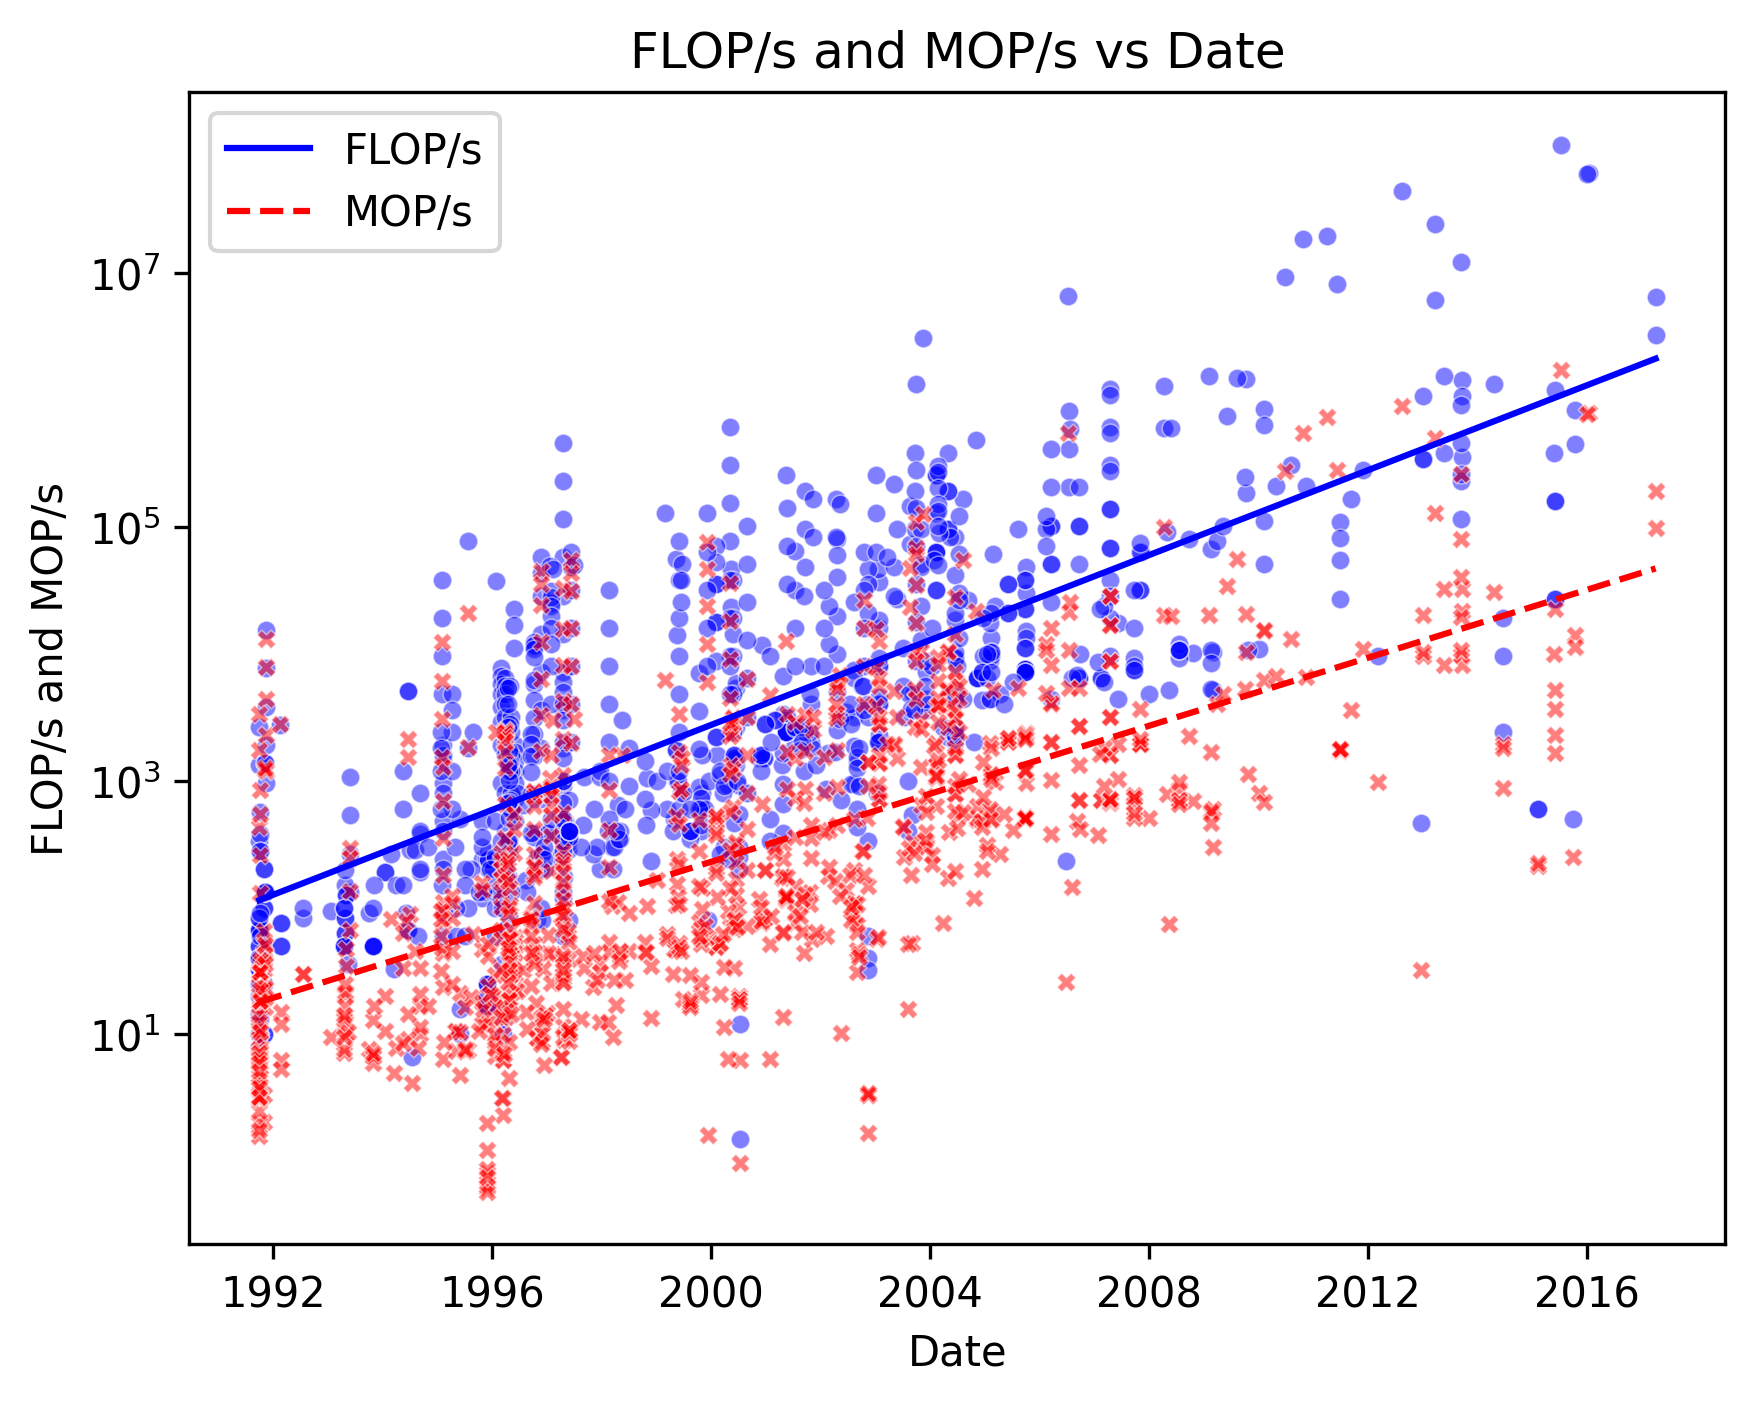
\includegraphics[width=\linewidth]{pictures/FLOPs_MOPs_vs_Date.png}
	\end{subfigure}
	\begin{subfigure}{.5\textwidth}
		\centering
		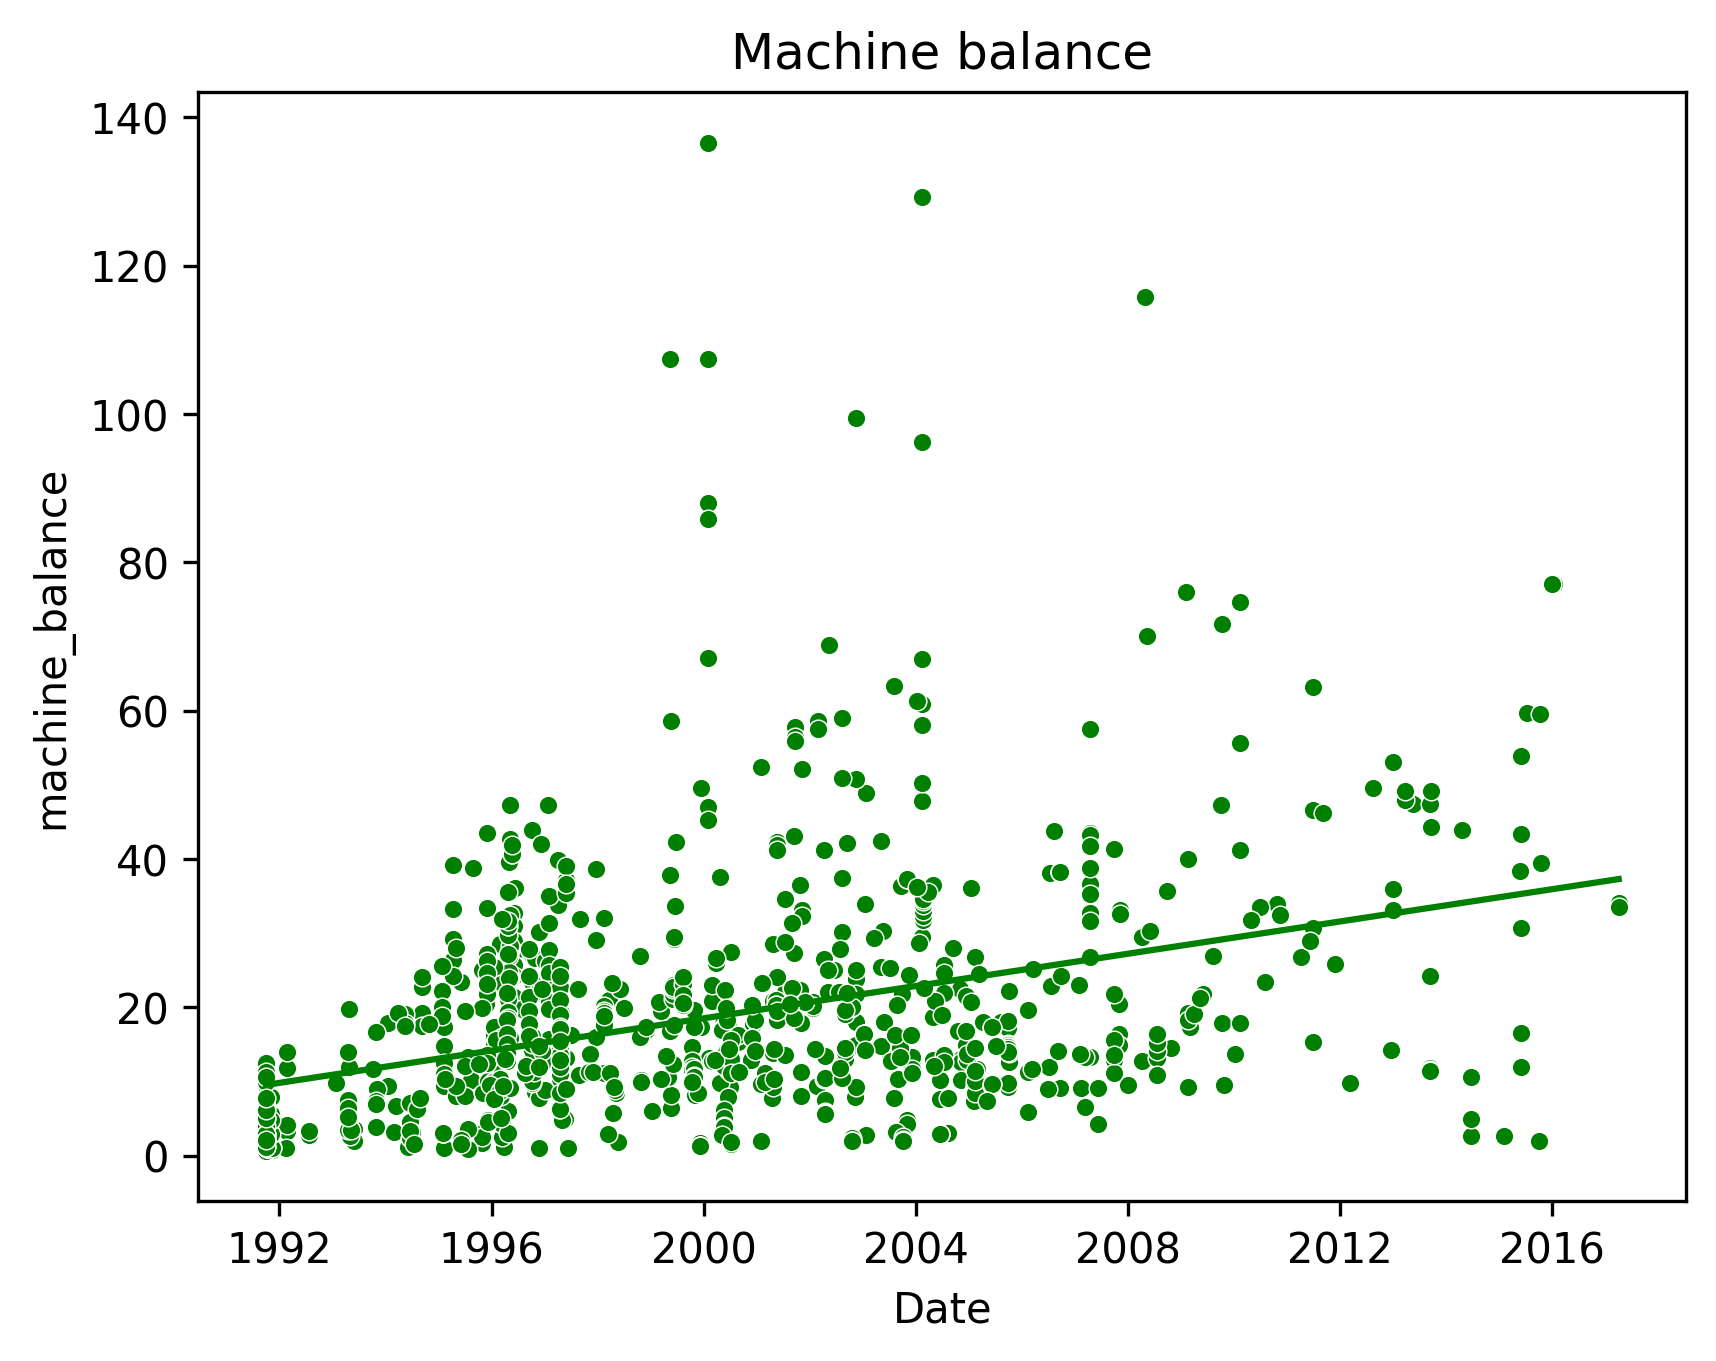
\includegraphics[width=\linewidth]{pictures/machine_balance.png}
	\end{subfigure}
	\caption{Illustration of the expanding Processor-Memory Gap. The left graph charts the progression of FLOPs and MOPs on a logarithmic scale across various computing platforms, with the FLOPs trendline demonstrating a steeper ascent, indicative of the widening gap. The right figure depicts the development of the machine balance score for these platforms.\protect\footnotemark{}}
	\label{fig:pmgap}
\end{figure*}
\footnotetext{Data was acquired from a collection of STREAM benchmark results on \url{https://www.cs.virginia.edu/stream/}.}

The increasing processor-memory performance gap becomes a critical problem when considering data access times. Take the equation for the average memory access time:
\begin{equation}\label{eq:avg_mem_time}
t_{avg} = p \cdot t_c + (1-p) \cdot t_m
\end{equation}
Here, $p \in \left[0,1\right)$ denotes the probability of a cache hit (Section \ref{sec:data_transfer}). As at least one instruction has to be fetched from memory, at least one cache miss per application is guaranteed, thus $p < 1$. $t_c$ and $t_m$ denote the times to access data from a cache and the main memory, respectively \cite{wulf1995hitting, mahapatra1999processor}. These times measure the performance of the cache and the main memory as a combination of memory latency and bandwidth (Section \ref{sec:data_transfer}). Without loss of generality, consider these times as the corresponding number of clock cycles.

As a result of the increasing processor-memory performance gap, $t_m$ (and to a lesser extent $t_c$) will be increasing exponentially, taking more and more clock cycles to access the same amount of data - clock cycles that could be used to perform calculations. As a result, the overall system performance will be increasingly determined by memory performance. At some point, CPUs would be able to execute code faster than we can feed them with instructions and data. For this reason, the processor-memory performance gap is also known as the memory wall problem \cite{wulf1995hitting, mckee2004reflections, mahapatra1999processor}.

To quantify the processor-memory performance gap, the notion of machine balance has been introduced \cite{mccalpin1997survey, mccalpin2016memory}:
\begin{equation}\label{eq:machine_balance}
	balance = \frac{peak\; FLOP/s}{sustained\; MOP/s}
\end{equation}
This metric, also depicted in Figure \ref{fig:pmgap}, is a measure of how well a system is balanced between computational and memory performance. A balance of 1 indicates a perfectly balanced system, whereas $balance \ll 1$ or $balance \gg 1$  indicates a system that is entirely compute or memory-bound, respectively \cite{mccalpin1997survey, mccalpin2016memory}.

\subsection{Computation and Memory Requirements}\label{sec:comp_mem_req}
Different applications have different requirements for system resources. There exist some programs that have a larger computational demand, thus benefiting from a higher machine balance (Section \ref{sec:pmgap}) \cite{mccalpin2016memory}. However, the memory wall problem states that it will be increasingly more difficult for such applications to exploit further advances in computational performance, as for any application the memory performance will grow to be the limiting factor \cite{wulf1995hitting, mckee2004reflections}.

Furthermore, we notice that computational as well as memory requirements are increasing rapidly. A prime example of this is the field of artificial intelligence systems, which currently sees exponential growth in the number of parameters used \cite{ourworldindata2023ai}. Hence, for any application, regardless of its computational or memory demands, significant strides must be made in enhancing both the processing and memory capabilities. This ensures that the constraints imposed by the memory wall problem do not inhibit the potential performance of these applications.

\subsection{Data Transfer Costs and Bottlenecks}\label{sec:data_transfer}
\paragraph*{Memory Latency} Memory latency pertains to the time delay between a request to access data from the main memory and the start of the execution of this operation. Increased memory latencies, measured in clock cycles, lead to the processor waiting longer for data, significantly tightening the performance bottleneck. This latency challenge can adversely impact the execution of applications, and its reduction is often a complex task \cite{machanick2002approaches}.
\paragraph*{Memory Bandwidth} Memory bandwidth denotes the volume for data transfer to or from memory per unit of time. A bottleneck arises when the bandwidth is insufficient to handle the required data transfer volume, causing the processor to wait for data \cite{machanick2002approaches}.
\paragraph*{Cache Misses}\label{sec:cache_misses} To alleviate the impact of memory latencies, a multi-tiered memory hierarchy has been implemented in modern computing systems. This hierarchy includes the use of caches, which are smaller, faster, and more expensive memory modules placed between the CPU and main memory. When the processor needs to access data, it first checks if the data is already in the cache, a situation known as a cache hit. However, if the data is not in the cache, the processor has to retrieve it from the slower main memory, a process known as a cache miss \cite{efnusheva2017survey, mahapatra1999processor, machanick2002approaches}. When a cache miss occurs, an entire block of memory known as a cache line is loaded into the cache. The cache line includes the requested data and some adjacent memory locations. However, this process of retrieving data from the main memory takes considerably more time due to the higher latency of the main memory. Therefore, cache management, handled by software, is vital to maintain optimal performance. Improper management can lead to an increase in cache misses, thereby significantly degrading the system's performance.

\subsection{Data Locality}\label{sec:data_locality}
Data locality is a key concept in enhancing memory performance and therefore reducing the implications of the processor-memory performance gap. It refers to the tendency of a processor to access the same set of memory locations, or closely stored memory locations, repetitively over a short period. This concept capitalizes on the multi-level memory hierarchy of modern computers: By improving data locality, one reduces the number of cache misses (Section \ref{sec:data_transfer}), i.e., decreases $p$ in Equation \ref{eq:avg_mem_time}, improving overall system performance \cite{unat2017trends, tate2014programming}.

There are two main types of data locality: temporal and spatial locality. Temporal locality involves reusing the same data within a relatively small duration. This means that if a memory location is accessed, it is probable that the same location will be accessed again soon. Spatial locality, on the other hand, refers to the use of data items stored in proximity. In other words, if a memory location is accessed, memory locations nearby will likely be accessed shortly \cite{esseghir1993improving}.

Data layout plays a significant role in the realization of data locality, as it can substantially influence the memory access patterns and hence, the underlying performance of a program. A thoughtful arrangement of data in memory can encourage both temporal and spatial locality, thus reducing cache misses and enhancing the overall system performance \cite{esseghir1993improving}.

To illustrate, consider a two-dimensional array laid out in memory, where elements in the same row are stored in consecutive memory locations. If an application iterates through this array row by row, it benefits from spatial locality, as loading one element of the matrix also loads the few next elements in the row into the cache due to loading of entire cache lines (Section \ref{sec:cache_misses}), thus reducing the number of cache misses. On the contrary, if the application were to traverse the array column by column, it would not benefit from spatial locality due to the dispersed memory locations of elements in the same column, leading to a higher rate of cache misses and reduced performance.

While this example demonstrates a simple scenario, the reality is often more complex, especially for larger and more intricate applications. Understanding the data access patterns of an application is key to deciding the best data layout, and this often requires an intimate knowledge of the program's structure. Moreover, optimizing data locality can be quite challenging due to the diversity of hardware architectures. The same program can exhibit different data locality characteristics on different hardware due to variations in the memory hierarchy (such as cache sizes and levels, memory bandwidth, and latency).

This paper will provide an overview of an approach to optimize data locality with the help of visualizations.
